% !TEX root = ../main.tex
\chapter{Implementation}
\label{Implementation}
In this section, how the design is implemented will be described in detail. 

\section*{Discrete Time Simulation Steps}
Demand and Generation requests are made and satisfied on a hourly basis. Due to the nature of Presage 2, actions and requests happen in discrete time steps. In this simulation, each hour has to be split into 5 discrete time-steps due to the out of order execution of Agent actions and the discrete time nature of Presage 2. What actions are performed in each of the time steps are outlined below:
\begin{enumerate}
	\item During the first time step, Agents submit their Generation and Demand requests to the Virtual Agent or Community they are part of.
	\item During the second time step, Virtual Agents or Communities aggregate the Generation and Demand requests received and submit their Generation and Demand requests to the Supervisor Agent
	\item During the third time step, the Supervisor Agent gathers the total Demand and Generation requests and subsequently allocates the Demand and Generation to the Virtual Agents
	\item During the fourth time step, the Virtual Agents or Communities receive the allocation given by the supervisor, and allocates that to the Agents
	\item During the 5th time step, the Agents appropriates the Demand and Generation allocation that has been given to them
\end{enumerate}

\section*{Agent Class Structure and Implementation}
Agents in Presage 2 are created by extending the \textit{AbstractParticipant} class as shown in the UML diagram in figure \ref{fig:AgentUML}. The class \textit{MasterAgent} is how a Supervisor Agent is defined within the Simulator. \textit{MasterAgent} is a simple class and is required to only do two things:
\begin{itemize}
	\item Keep track of the Virtual Agents in the community it is reponsible for
	\item Allocating the correct amount of Demand and Generation to the Virtual Agents
\end{itemize}

To satisfy those requirements the following methods in the class are implemented:
\begin{itemize}
	\item \textit{addChild()} method is used for keeping track of the Virtual Agents. This is called during the initial Simulation set-up as part of the Agent creation and initialisation process.
	\item \textit{step(int)} method is called by Presage during the simulation to allow the Agent to act on the environment. Demand and Generation are allocated to the Virtual Agents when this method is called automatically by Presage
\end{itemize}

A Virtual Agent (\textit{ParentAgent} class) is a more advanced \textit{MasterAgent}. It is required to:
\begin{itemize}
	\item Keep track of which Agent is the Supervisor Agent
	\item Keep track of the Agents that depend on it to submit Demand and Generation requests on their behalf
	\item Submit Generation and Demand requests to the Supervisor Agent it is connected to
	\item Allocating the correct amount of Demand and Generation to the Agents
\end{itemize}

To perform the duties outlined above, the following methods are implemented:
\begin{itemize}
	\item The \textit{constructor} of this object is responsible for keeping track of which Agent is the Supervisor Agent. The \textit{constructor} is called when this object is created in the initial Simulation set-up as part of the Agent creation and initialisation process.
	\item \textit{addChild()} method is used for keeping track of the Agents. This is also called during the initial Simulation set-up as part of the Agent creation and initialisation process.
	\item \textit{step(int)} method is called by Presage during the simulation to allow the Agent to act on the environment. Demand and Generation requests are sent to the supervisor, and allocation of Demand and Generation are also made to the Agents when this method is called automatically by Presage.
\end{itemize}

Prosumer Agents are Virtual Agents but with no aggregation function, as a Prosumer Agent is the most elementary Agent is the most elementary Agent or sub-community in this holonic system simulation. A Prosumer Agent is required to:
\begin{itemize}
	\item Keep track of which Agent is the Virtual Agent
	\item Submit Generation and Demand requests to the Virtual Agent it is connected to
	\item Appropriate the allocated amount of Generation and Demand allocated
\end{itemize}

The Prosumer Agent is implemented with the following methods to allow it to perform the requirements outlined above:
\begin{itemize}
	\item The \textit{constructor} of this object is responsible for keeping track of which Agent is its \textit{ParentAgent}. The \textit{constructor} is called when this object is created in the initial Simulation set-up as part of the Agent creation and initialisation process.
	\item \textit{addChild()} method is used for keeping track of the Agents. This is called during the initial Simulation set-up as part of the Agent creation and initialisation process.
	\item \textit{step(int)} method is called by Presage during the simulation to allow the Agent to act on the environment. Demand and Generation requests are sent to the supervisor, and allocation of Demand and Generation are also made to the Agents when this method is called automatically by Presage.
	\item \textit{addProductivity(), addSocialUtility(), addProfileHourly()} are the methods that are called during the initial Simulation set-up as part of the Agent creation and initialisation process to define the properties of this Agent.
\end{itemize}


\begin{figure}[!h]
	\centering
	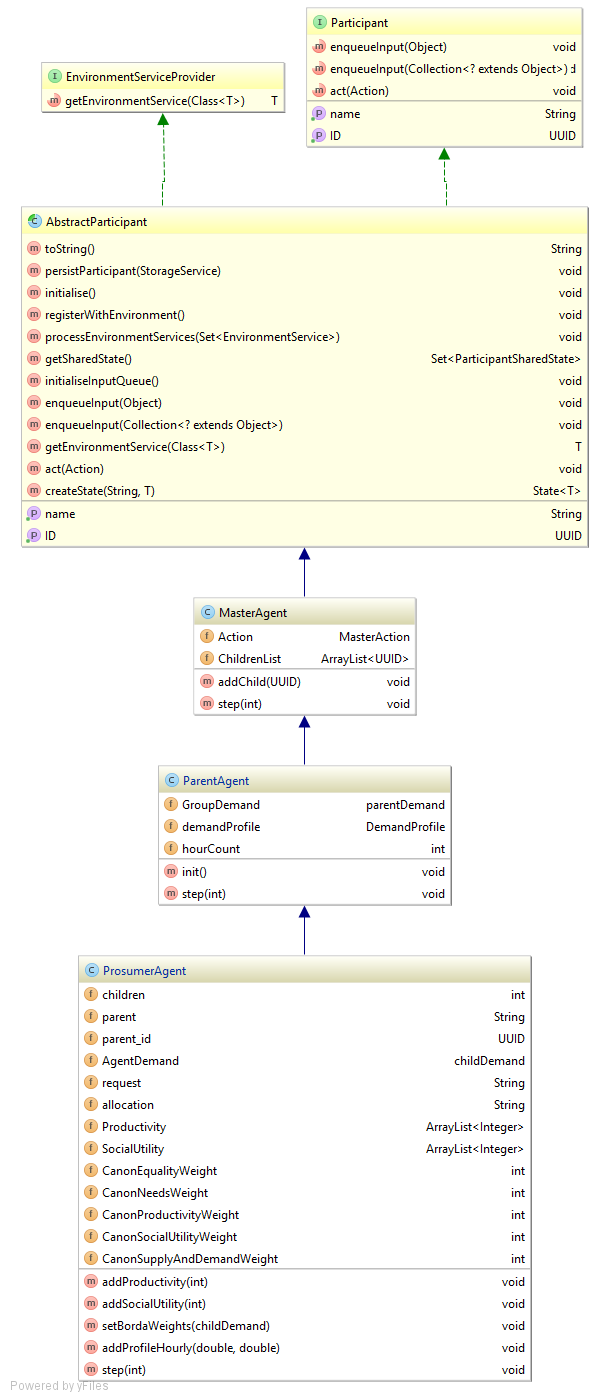
\includegraphics[scale=0.4]{Images/AgentUMLEdited.png}
	\caption{Agent UML Diagram}
	\label{fig:AgentUML}
\end{figure}


\clearpage


\section*{Environment Services}

All Agents perform actions on Environments, which contains one or more "shared states". In Presage 2, all communication that happens between Agents are done via the environment by storing the data in a "shared state". In the context of this simulation shared state would be information such as Demand and Generation requests or the amount available in the Common Resource Pool. A visual diagram on how the Environment classes in this simulation are implemented can be found in figures \ref{fig:ServiceUML} and \ref{fig:ServiceUML2}.

\subsection*{Global Environment Service}
All Agents are registered to the Global Environment Service, \textit{GlobalEnvService} class. Like all Environment service classes in Presage, this was extended from the \textit{EnvironmentService} class built into Presage. This class contains all of the methods that are called when allocations are being made. During time step 3 of a simulated hour, the \textit{allocate()} method is called from the \textit{MasterActionHandler} to perform allocations on behalf of the Supervisor Agent. \textit{allocate()} method by default satisfies all the requirements of connected Virtual Agents if there is enough Generation to support it. If there is excess Generation, the excess is curtailed proportionally. 
If however, there isn't enough Generation, method \textit{allocate\_fairly()} is called, and the Virtual Agents are ranked according to the five applicable \textit{Rescher's Canons of Distributive Justice}. These rankings are computed by calling the methods such as \textit{canon\_of\_equality()}. The allocations are stored in the \textit{PowerPoolEnvService}.
At the end of the allocation process, the data about the allocation is stored in the environment ready for time step 3 of the next simulated hour via the method \textit{environmentStore}.

\begin{figure}[!h]
	\centering
	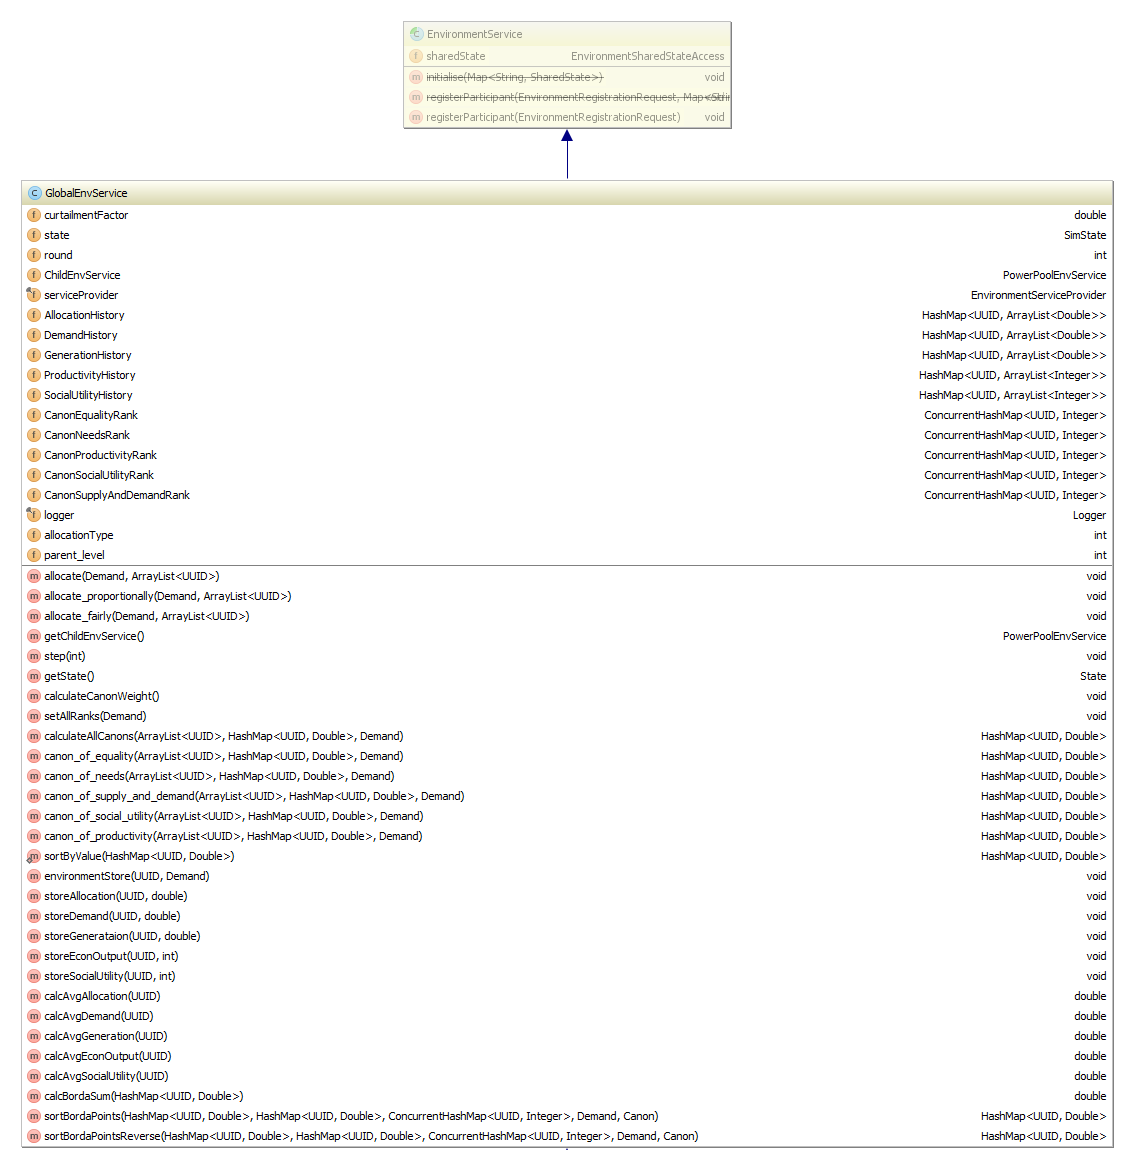
\includegraphics[scale=0.3]{Images/EnvironmentUML-1.png}
	\caption{Environment Services UML Diagram}
	\label{fig:ServiceUML}
\end{figure}


\subsection*{Supervisor Environment Service}
The \textit{PowerPoolEnvService} is the Environment Service accessible by both the Supervisor Agent and the Virtual Agents. The \textit{PowerPoolEnvService} inherits from \textit{GlobalEnvService} class, and does a lot of the same things on a smaller scale.  The \textit{PowerPoolEnvService} is used to store information about the Virtual Agents, such as their aggregated Demand and Generation requests, and contains the same methods that are called when allocations are being made by the Virtual Agents. During time step 2 of a simulated hour, Virtual Agents sum up their Prosumer Agent Demand and Generation requests, and store them in \textit{PowerPoolEnvService}. During time step 4 of a simulated hour, the \textit{allocate()} method is called from the \textit{parentDemandHandler}. \textit{allocate()} method by default satisfies all the requirements of Agents if there is enough Generation to support it. If there is excess Generation, the excess is curtailed proportionally. In a holonic system, Agents are not able to access information concerning other Agents that it is not directly connected to. A separate Environment Service is used to prevent the Supervisor Agent from being able to access and modify "shared states" about Prosumer Agents that are not directly connected to the Supervisor Agent.

Simiar to the \textit{GlobalEnvService} class, if there isn't enough Generation, method \textit{allocate\_fairly()} is called, and the Agents are ranked according to the five applicable \textit{Rescher's Canons of Distributive Justice}. These rankings are computed by calling the methods such as \textit{canon\_of\_equality()} which are inherrited from the \textit{GlobalEnvService}. \textit{PowerPoolEnvService} contains \textit{Overriding} \textit{allocate()} and textit{allocate\_fairly()} methods and do not inherrit these from the \textit{GlobalEnvService}, because the allocation data is required to be stored in the \textit{ParentEnvService}. At the end of the allocation process, the data about the allocation is stored in the environment ready for time step 4 of the next simulated hour via the method \textit{environmentStore}.

\begin{figure}[!h]
	\centering
	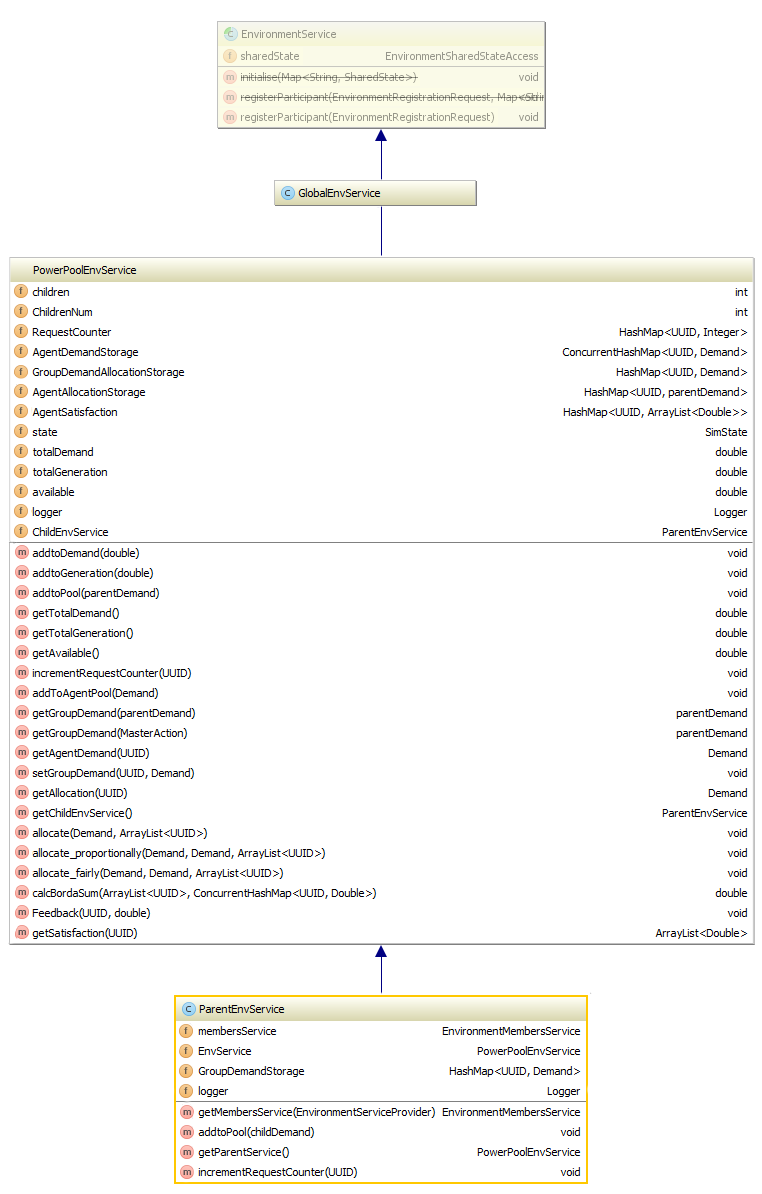
\includegraphics[scale=0.3]{Images/EnvironmentUML-2.png}
	\caption{Environment Services UML Diagram}
	\label{fig:ServiceUML2}
\end{figure}

\subsection*{Virtual Agent Environment Service}
The \textit{ParentEnvService} is the Environment Service accessible by both the Virtual Agents and the Prosumer Agents. The \textit{ParentEnvService} inherits from the \textit{PowerPoolEnvService}, and does the same things on a smaller scale. The \textit{ParentEnvService} is used to store information about the Prosumer Agents, such as their individual Demand and Generation requests, and also contain information about their allocations. During time step 1 of a simulated hour, Agents store their Demand and Generation requests in this Environment Service as a "shared state". During time step 2 of a simulated hour, Virtual Agents aggregate the stored Demand and Generation requests and store them in the \textit{PowerPoolEnvService}. During time step 5, Agents retrieve their allocations from \textit{ParentEnvService}.

\subsection*{Action}
To act on the Environment or acess a shared state in the Environment, Agents are expected to perform an Action. In the context of this simulation, Action would be Demand/Generation requests. As Generation can be modelled as a negative Demand, a single Action can be defined to allow the contribution and appropriation of electricity. 

\begin{figure}[!h]
	\centering
	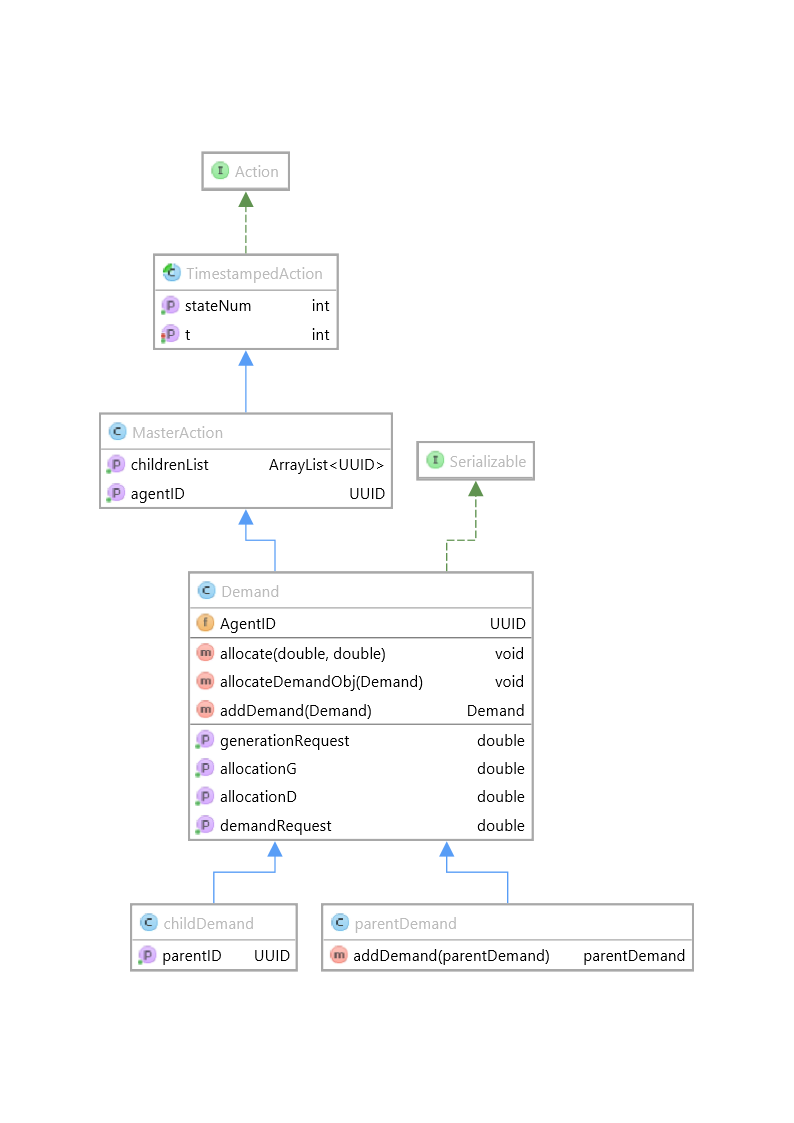
\includegraphics[scale=0.5]{Images/ActionUML.png}
	\caption{Actions UML Diagram}
	\label{fig:ActionUML}
\end{figure}

\subsection*{Action Handlers} % (fold)
To enable the Environment to be able to process the Action requests, Action Handlers need to be created to tell the simulation how to deal with Actions from Agents.

\begin{figure}[!h]
	\centering
	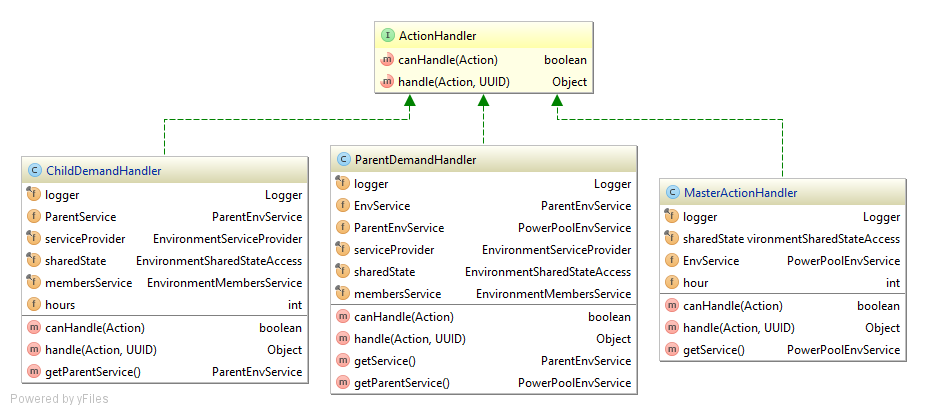
\includegraphics[scale=0.4]{Images/ActionHandlerUML.png}
	\caption{Action Handler UML Diagram}
	\label{fig:ActionHandlerUML}
\end{figure}
% subsubsection subsubsection_name (end)

\subsection*{Simulation}


\section*{Issues}
Out of order parallel execution meant that Agents need to submit their individual Demands to the SharedState, and have that summed at the end of each timestep. It is not possible to sum the Demands on the fly.

Being new to both Java and Presage presented problems of its own. It was difficult to understand how simulations could be run and therefore create our own.

One action per time step meant that it takes 4 time steps to simulate one round of request and appropriation of electricity. It would therefore take 24*4 time steps to simulate a full day of requests and appropriation.

Difficulty with initialising Agents with arrays meant that Agents had to be created with no Demand or Generation Profiles, and the Demand and Generation Profiles were added one by one via a for-loop and the addProfileHourly() method.


